% 1977 年湖南株洲卷第 9（1）题：三个半径都是 R 的圆两两外切；圆心三角形 ABC（等边），
% 切点 D 在 AB 上、F 在 AC 上、E 在 BC 上，中间曲边三角形加阴影（按源卷第 4 页布局）
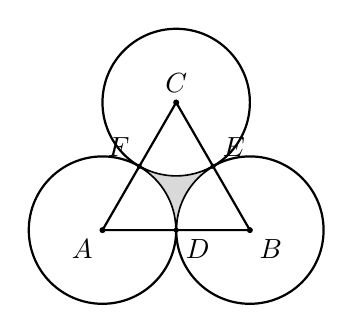
\begin{tikzpicture}[scale=0.78]
  \coordinate (A) at (0,0);
  \coordinate (B) at (2.4,0);
  \coordinate (C) at (1.2,2.078);
  \draw[thick] (A)--(B)--(C)--cycle;
  \draw[thick] (A) circle (1.2);
  \draw[thick] (B) circle (1.2);
  \draw[thick] (C) circle (1.2);
  \filldraw[fill=black!15] (1.2,0) arc (0:60:1.2) arc (240:300:1.2) arc (120:180:1.2) -- cycle;
  \fill (A) circle (1.4pt) node[below left] {$A$};
  \fill (B) circle (1.4pt) node[below right] {$B$};
  \fill (C) circle (1.4pt) node[above] {$C$};
  \fill (1.2,0) circle (1.2pt) node[below right] {$D$};
  \fill (0.6,1.039) circle (1.2pt) node[above left] {$F$};
  \fill (1.8,1.039) circle (1.2pt) node[above right] {$E$};
\end{tikzpicture}
